\documentclass[conference]{IEEEtran}
\usepackage{cite}
\usepackage{amsmath,amssymb,amsfonts}
\usepackage{algorithm}
\usepackage[noend]{algpseudocode}
\usepackage{float}
\usepackage{graphicx}
\usepackage{caption}
\usepackage{subcaption}
\usepackage{textcomp}
\usepackage{xcolor}
\usepackage[utf8]{inputenc}
\def\BibTeX{{\rm B\kern-.05em{\sc i\kern-.025em b}\kern-.08em
    T\kern-.1667em\lower.7ex\hbox{E}\kern-.125emX}}
\bstctlcite{IEEEexample:BSTcontrol}
\graphicspath{{./}{figures/}}


\begin{document}

\title{Comparisons Between Parallel Octree Implementations
}

\author{\IEEEauthorblockN{Katherine Abreu, 
Alexandra Brown, 
Ryan Bugge,  
and Ayiana Mallory}

\IEEEauthorblockA{
College of Engineering and Computer Science\\
University of Central Florida, Orlando, Florida 32816\\
}}


\maketitle

\begin{abstract}
Octrees are tree data structures where each node has eight children nodes, or octants. They are commonly used for three-dimensional modeling and real-world problem solving where binary trees and quadtrees may fall short. In this paper, we have implemented a pointer-based octree using standard representation. We tested four different methods of synchronization, including coarse-grained, fine-grained, optimistic, and non-blocking synchronization. Our targeted problem involved finding an efficient parallel technique when it came to adding, searching, and removing nodes in octrees with the goal of having a lock-free octree implementation. Of the parallelization methods tested, our optimistic approach outperformed all of the other approaches, leading to speedups of about 2.6 times for removal, 4.6 times for insertion, and 2.2 times for mixed operations. 

\end{abstract}

\begin{IEEEkeywords}
parallel computing, octrees, locking
\end{IEEEkeywords}

\section{Introduction} \label{sec:sec1}

Octrees are tree data structures where each node has either eight children nodes or no children nodes at all. If they don't have any children, they are known as leaf nodes. In this case, each of the children nodes are known as octants. Octrees have many applications in three-dimensional computer graphics and can be used to represent the three-dimensional world. They can be defined as a “recursive, axis-aligned, spatial partitioning data structure” \cite[para. 1]{octrees1} which helps optimize collision detection and nearest neighbor search. In other words, they allow us to locate the closest points from a given point as well as focus on a certain area in an optimal way. They are tree data structures with the purpose of subdividing into octants to split a three-dimensional space.

In this paper, we aim to find the most efficient way to implement and utilize octrees with parallel computing. We have implemented four methods of synchronization including coarse-grained, fine-grained, optimistic, and non-blocking synchronization. 

The rest of this paper is organized as follows: Section \ref{sec:sec2} is about previous works involving multi-threading with octrees. Section \ref{sec:sec3} discusses the ways to implement octrees and the algorithms utilized for our research. Section \ref{sec:sec4} describes the different methods of parallelization used and how we implemented them. Section \ref{sec:sec5} discusses our results of testing each parallelization method. Section \ref{sec:sec6} compares our results with expected results and considers areas of further investigation.


\section{Related Works} \label{sec:sec2}
In 1992, Chaudhary et al. \cite{ChaudharyEtAl} presented methods for constructing and manipulating octrees in parallel machines. To construct the octree, they continually split a binary image into octants until each node was either all white (object) or black (non-object). To parallelize the octree, it was treated as three quadtrees, representing the top, front, and side views of a 3D object,  traversed in parallel. They achieved a slight speedup in comparison to the sequential version. However, they did experience a bottleneck when it came to task creation and shared resources.

In 2005, Hariharan and Aluru \cite{HariharanAluru} discussed software for parallelizing compressed octrees. The octrees were stored in a postorder traversal order and load balancing was not required. Using their method, they saw good speedup regardless of whether or not the distribution was uniform and it scaled well with the number of processors being used. 

In 2010, Zhou et al. \cite{ZhouEtAl} presented the first parallel surface reconstruction algorithm that ran on the GPU. It used an octree to reconstruct a real-world 3D scan. Their octree implementation consisted of four arrays: vertex array, edge array, face array, and node array. The GPU implementation performed over two orders of magnitude better than a similar CPU implementation. Due to memory constraints, however, the octree could only have a depth of nine. 

In 2012, Tero Karras \cite{Karras} implemented an in-place algorithm for radix-binary trees used to construct octrees on the GPU. It outputted nodes in a strict depth-first order and scaled well, as well as performed better than other generation methods tested by avoiding sequential bottlenecks. 

This is by no means a comprehensive review of the work done on octrees, but it provided insight on the types of results we expected to see. 

\section{Octree Implementation} \label{sec:sec3}
There are generally two different types of octree data structures. They can be pointer-based octrees or linear-based octrees with certain advantages and disadvantages in each case. Both pointer-based and linear-based have a node structure that contains a pointer of all the objects a node encloses. They also have an Axis Aligned Bounding Box which is stored as two vectors called \textbf{Center} and \textbf{HalfSize} to represent the volume. They store the center and edge of the Axis Aligned Bounding Box, respectively \cite{octrees2}. We decided to focus on pointer-based octrees because it allowed us to traverse and update the octree in a quick and efficient way, allowing us to implement the parallel techniques we chose to incorporate. Having threads that continuously add, remove, and search concurrently will cause an octree to be updated frequently. Therefore, we decided pointer-based was the best choice.

There are three different ways to represent pointer-based octrees. One way is called \textit{standard representation}. It involves having a pointer for each of the eight child nodes with the option of having a pointer for the parent node. This method also uses a Boolean flag, which can be called \textbf{isLeaf}. Its purpose is to allow us to know if the nodes are either inner nodes or leaf nodes. It also allows for on-demand allocation, meaning they don't need to allocate memory for all eight children at the same time, allowing us to save memory. Generally, it also takes up to 105 bytes of storage space \cite{octrees2}.

Another type of representation is \textit{block representation}, which is similar to standard, except it involves storing a pointer to all eight children rather than having one pointer for each of them. “That way the storage size of an inner node can be reduced from 105 bytes down to 49 bytes” \cite[para. 7]{octrees2}. This ends up being only 47 percent of the original storage size. It also uses a Boolean flag and has the option of having a pointer for the parent node. The disadvantage is that it does not support on-demand allocation, since it would have to allocate all eight children every time a node is subdivided. In a way, it's like all eight children are one block, hence the name \cite{octrees2}.

The last type of representation is \textit{sibling-child representation}. Compared to standard representation, each octant only uses two pointers instead of eight. For example, given a created node, according to its node structure, the first pointer, \textbf{NextSibling}, points to the next child node that shares the same parent. The second pointer, \textbf{FirstChild}, points to the first child node of the node we have just created. This only ends up using one-fourth of the memory used for pointers, since it uses two pointers instead of eight. A consequence of using this is that it ends up “dereferencing on average four times more pointers” \cite{octrees2} when nodes are randomly accessed instead of sequentially. It also uses a Boolean flag and allows for on-demand allocation\cite{octrees2}.

Out of all the three choices, we ended up using the standard representation. By using eight pointers for all eight child nodes, we were able to use on-demand allocation, meaning a child node only needed to be allocated when we found an object that needed to be located there. This was better than having to allocate all eight children every time, which would have led to memory waste.  We also had the advantage of being able to update and traverse it easily and quickly by using all eight pointers, which was beneficial and crucial when working with concurrent threads. Block representation would have led to too much memory waste since there could have been many empty child nodes. Even though modifying and traversing the list would have been just as easy as the standard representation. In the case of the sibling-child representation, it would have ended up saving a lot of memory, but because of the way the pointers would have been set up, traversing it would have been complicated and slow, which wouldn't have correlated well with concurrent threads. Therefore, at the end, it depended on whether memory usage or traversal speed was important. In this case for us, it was traversal speed, since we were dealing with many threads that were adding, removing, and searching the octree concurrently. Thus, standard representation was the best option.

\subsection{Algorithms Implemented}

There were four algorithms we ended up using. They involved finding the location of the correct node, inserting points into the octree, subdividing a node, and resizing the octree without having predetermined bounds. Throughout all of the algorithms, we also incorporated Morton codes, also known as z-order curves, which involves positioning nodes inside of other nodes. Morton codes first denote the location of a node inside its parent node by using three bits to represent the three dimensions. The first bit is used for the x-axis, the second is for the y-axis, and the third is for the z-axis. Therefore, there are eight possible different values which go from zero to seven. For our pointer-based octree, these values were used to represent the index in the array that stored pointers to the parent node’s children.

For the find algorithm, which can be observed in Algorithm \ref{alg:octree find}, we take a point as input and output the correct node. In this case, instead of using the Morton codes directly, we translate it into an integer between zero and seven, which allows us to use it as an index to the children’s array and store it in \textbf{next}. Every time it starts back at the beginning of the while loop, \textbf{next} is set to zero to get the new index. The way the algorithm works is that in the beginning, we set the current node to the root node and traverse the list until we encounter the leaf node. We know where to traverse to by comparing the x, y, and z values of the point to the values of the current node in order to know which location in the children’s array the current node should traverse to. Once we encounter the leaf node, we return that current node. We know whether the current node is a leaf node by checking \textbf{curr.isLeaf}, which is the Boolean flag in the node structure.

\setcounter{algorithm}{0}
\begin{algorithm}[h]
    \caption{Find}\label{alg:octree find}
    \begin{algorithmic}[1]
        \Statex \textbf{Input:} Point
        \Statex \textbf{Output:} Node
        \State {curr $\leftarrow$ root}
        \While {!curr.isLeaf}
        \State next $\leftarrow$ 0
        \If {Point.x $\geq$ curr.center.x}
        \State next $\leftarrow$ next + 4
        \EndIf
        \If {Point.y $\geq$ curr.center.y}
        \State next $\leftarrow$ next + 2
        \EndIf
        \If {Point.z $\geq$ curr.center.z}
        \State next $\leftarrow$ next + 1
        \EndIf
        \State curr $\leftarrow$ curr.children[next]
        \EndWhile
        \State \Return curr
    \end{algorithmic}
\end{algorithm}

In the insertion algorithm, depicted in Algorithm \ref{alg:octree insert}, we also take a point as input and output a Boolean result. In this algorithm, we call \verb|find()|, and as stated before, \verb|find()| returns the node with the proper location. Afterwards, we check if the node contains the point already. If it does, we return false. Otherwise, we insert the point into the node. Finally, we check if we need to subdivide the node by checking if the size of the children exceeds the limit. In this case, we don’t use a depth limit and instead we use a limit to the number of points an octree can have. The contains and remove algorithms are also quite similar to the insertion algorithm and behave almost the same way. The only difference is that we remove the point or check if the point is located at the node rather than insert it.

\begin{algorithm}[h]
    \caption{Insert}\label{alg:octree insert}
    \begin{algorithmic}[1]
        \Statex \textbf{Input:} Point
        \Statex \textbf{Output:} Boolean
        \State {node $\leftarrow$ find(Point)}
        \If {node.contains(Point)}
        \State \Return False
        \EndIf
        \State {node.points.add(Point)}
        \If {node.points.size $\geq$ limit}
        \State node.subdivide
        \EndIf
        \State \Return True
    \end{algorithmic}
\end{algorithm}

The subdivision algorithm doesn’t take any input or produce any output. In this case, we first mark the Boolean flag, \textbf{isLeaf}, to false, so that the current node is no longer a leaf node, since high principle leaf nodes do not contain children. Next, we calculate the new half size of the node’s children, which is just the current \textbf{halfSize} divided by two, and store it into \textbf{newHalfSize}. We can then calculate the center of each child node by using the variables in the three nested for loops as shown in Algorithm \ref{alg:octree subdivide}. Each dimension has a specific formula where all three follow the same structure. The only difference is the value they obtain from \textbf{center} and whether they are using the \textbf{i} value, the \textbf{j} value, or the \textbf{k} value from the nested loops. It’s these three nested for-loops that allow us to obtain the Morton code. From there, the children’s array is populated with new nodes that are initialized using the new center positions, which were stored in \textbf{X}, \textbf{Y}, and \textbf{Z}, as well as \textbf{newHalfSize}. Next, every point in the current node needs to be removed and re-inserted back into the child node it belongs in. This section follows a similar structure to the find algorithm where it first needs to locate the index of the children's array by using the \textbf{x}, \textbf{y}, and \textbf{z} values.

\begin{algorithm}[h]
    \caption{Node Subdivision}\label{alg:octree subdivide}
    \begin{algorithmic}[1]
        \State isLeaf $\leftarrow$ False
        \State newHalfSize $\leftarrow$ halfSize $\div$ 2
        \For {i $\in$ \{0, 1\} }
        \For {j $\in$ \{0, 1\} }
        \For {k $\in$ \{0, 1\} }
        \State X $\leftarrow$ center.x - newHalfSize + i $\times$ halfSize
        \State Y $\leftarrow$ center.y - newHalfSize + j $\times$ halfSize
        \State Z $\leftarrow$ center.z - newHalfSize + k $\times$ halfSize
        \State children[i $\times$ 4 + j $\times$ 2 + k] $\leftarrow$ Node(\{X, Y, Z\}, newHalfSize)
        \EndFor
        \EndFor
        \EndFor
        \ForAll {Points \textbf{in} Node}
        \State remove(Point)
        \State next $\leftarrow$ 0
        \If {Point.x $\geq$ center.x}
        \State next $\leftarrow$ next + 4
        \EndIf
        \If {Point.y $\geq$ center.y}
        \State next $\leftarrow$ next + 2
        \EndIf
        \If {Point.z $\geq$ center.z}
        \State next $\leftarrow$ next + 1
        \EndIf
        \State children[next].points.add(Point)
        \EndFor
    \end{algorithmic}
\end{algorithm}


Lastly, we also have a resize algorithm, which is used when the bounds are not precomputed beforehand. This is depicted in Algorithm \ref{alg:octree resize}. Because this algorithm was difficult to implement for concurrency, for each synchronization method we focused on, we had two versions. Version one involved the resizing algorithm and version two involved using precomputed bounds. Therefore, this resizing algorithm was only used for the synchronization methods we coded in version one. In this algorithm, we take a point as input and produce no output. The first thing we do is check if the point is out of bounds. If it is, the octree must continually resize until it can fit the point. Once we know the point is out of bounds, we need to determine the direction the point has in relation to the center of the octree. In this case, instead of using the Morton code for the direction of the point, we initially set the values in the variable, \textbf{direction}, with ones. From there, based on the comparisons of the values in \textbf{Point} with the values in \textbf{root.center}, those in \textbf{direction} get set to negative one. Within that same step, we also calculate the Morton code so that we designate a location that the current root will have inside of the new root we are creating. Since we always expand the octree towards the point, the Morton code of the current root is always in the opposite direction of the expansion. The new root is then subdivided in order to initialize its children. It follows a similar approach to the subdivision algorithm. The only difference is that in their formulas they focus on the values of the current root and the values of the direction when subdividing. We then use the \textbf{rootCode} of the current root and replace the corresponding node in the child array with the current root. Finally, at the end of resizing, we replace the octree’s root pointer with the newly created root. Since the point may still reside outside of the resized octree, the process is repeated until the point is finally within bounds of the root node.

\begin{algorithm}[h]
    \caption{Resize}\label{alg:octree resize}
    \begin{algorithmic}[1]
        \Statex \textbf{Input:} Point
        \While {Point is out of bounds}
        \If {Point.x $<$ root.center.x}
        \State direction.x $\leftarrow$ -1
        \EndIf
        \If {Point.y $<$ root.center.x}
        \State direction.y $\leftarrow$ -1
        \EndIf
        \If {Point.z $<$ root.center.x}
        \State direction.z $\leftarrow$ -1
        \EndIf

        \State newHalfSize $\leftarrow$ root.halfSize $\times$ 2;
        \State newCenter.x $\leftarrow$ root.center.x + direction.x $\times$ root.halfSize
        \State newCenter.y $\leftarrow$ root.center.y + direction.y $\times$ root.halfSize
        \State newCenter.z $\leftarrow$ root.center.z + direction.z $\times$ root.halfSize
        \State newRoot $\leftarrow$ Node(NULL, newCenter, newHalfSize)
        \State newRoot.subdivide
        \State rootCode $\leftarrow$ (direction.x + 1) $\times$ 2
        \State rootCode $\leftarrow$ rootCode + (direction.y + 1)
        \State rootCode $\leftarrow$ rootCode + (direction.z + 1) $\div$ 2
        \State newRoot.children[rootCode] $\leftarrow$ root
        \State root $\leftarrow$ newRoot
        \EndWhile
    \end{algorithmic}
\end{algorithm}

\section{Methods of Parallelization} \label{sec:sec4}

As stated before, we tested the concurrency of adding, removing, and searching in octrees by testing it with four synchronization methods: coarse-grained, fine-grained, optimistic, and non-blocking.

\subsection{Coarse-Grained Synchronization}
The coarse-grained synchronization algorithm is essentially a sequential algorithm and it involves the use of only one lock. Each thread must acquire the lock before it is able to access the list of items. After the thread locks the object, it can begin execution. Afterward, it releases the lock, ready for another thread to access the list. Thus, the linearization point for any method call is the moment the thread obtains the lock. This is essentially used for all types of method calls, such as \verb|add()|, \verb|remove()|, and \verb|contains()| \cite{textbook}.

\subsubsection{Our Implementation}~\\
\indent \indent We decided to follow a similar approach when implementing the coarse-grained synchronization method into our program. In our method, every time a thread calls \verb|insert()|, \verb|remove()|, or \verb|contains()|, it attempts to acquire the lock. Once it has the lock, it acts as a signal that they have locked the entire octree. Once the thread is done adding, removing, or searching for an object, it releases the lock. 

\indent \indent As mentioned before, we implemented two versions of this. Version one uses \verb|resize()| whereas version two uses precomputed bounds. In this case, both versions utilized the same approach above. The only difference is that version one calls the \verb|resize()| function inside of \verb|insert()| after acquiring the lock and before inserting the point to check if it needs to be resized before inserting. It also allows the thread to resize before any other thread locks the octree.

\indent \indent To make this more optimal, for both versions, we added a finally block at the end to guarantee that the thread will release the lock no matter what happens after the try block exits. This ensures that even in the case of an exception being thrown, the thread will still release the lock. This was an easy implementation and is considered to be correct with an average runtime of 2.20 seconds for version one and an average runtime of 2 seconds for version two when doing insertion and removal with twelve threads. The problem is that it doesn't bode well with contention. A bottleneck can occur with the issue that if one thread gets delayed, the rest of the threads will be delayed as well. We expected this runtime to be worse compared to the other parallel techniques we implemented.

\subsection{Fine-Grained Synchronization}
Fine-grained synchronization is similar to coarse-grained synchronization with the exception that, instead of locking the entire list, each thread traverses through the list using two locks: one for the predecessor and one for the current node. All the threads are able to go down the list together and only lock individual nodes in the list. It involves a few more rules with the way they are locked. Once the predecessor is locked, the current node can be locked as well, but only while the predecessor remains locked. If the predecessor is unlocked and then the current node is locked, there’s a chance another thread could delete that current node or insert another node in between before the current node is locked. Another name for this is lock coupling. All of the methods must also lock in the same order to avoid deadlock \cite{textbook}.

This type of synchronization is deadlock-free as well as starvation-free. As stated before, deadlock is avoided because all the methods lock the predecessor and current node in the same order, which in this case, is predecessor and then current node. Let’s say there are two nodes \textit{a} and \textit{b} where \textit{a} points to \textit{b} and let’s say the \verb|delete()| function is set to have the thread lock the current node and then lock the predecessor while the \verb|add()| function is set to have the thread lock the predecessor and then the current node. If a thread calls \verb|delete()| and locks node \textit{b} while another thread calls \verb|add()| and locks node \textit{a}, the first thread will forever wait for node \textit{a} to unlock while the second thread will forever wait for node \textit{b} to unlock, resulting in a deadlock. Since fine-grained synchronization makes sure that each method locks in the same order, deadlock-freedom is achieved. Starvation-freedom is also achieved since the threads go down the line with no deadlock. One thread will never starve from locking a node because no matter what happens, the threads must unlock at some point and continue down the line. This is especially true because of the finally block in the implementation that guarantees the threads will unlock even if an exception occurs \cite{textbook}.

\subsubsection{Our Implementation}~\\
\indent \indent We also followed a similar approach in both of our versions of fine-grained synchronization. Both versions involve using a predecessor and a current node. The current node gets set to root and once it's locked, we find the next location in the octree. Once we do, we set the predecessor to current, so that the predecessor will now be locked. Then, once we set current to the next location, we lock the current node and then unlock the predecessor, starting the cycle again. This happens for \verb|contains()| and \verb|remove()| for both versions. This also happens for \verb|insert()| in version two.

 \indent \indent For \verb|insert()| in version one, things are a little different, since it involves \verb|resize()|. In this case, for version one, instead of locking the root right away, both \verb|insert()| and \verb|resize()| start in a while loop if it hasn't been able to lock the root in order to make sure that if a thread is in the middle of resizing, the thread trying to insert will have to wait and vice versa.

\indent \indent Similar to coarse-grained synchronization, we also followed a similar pattern to optimize it. We added a finally block for both versions in order to make sure that no matter what happens, the thread will release the lock. With this implementation, we had an average runtime of about 5.0 seconds in version one and an average runtime of about 3.20 seconds in version two when doing insertion and removal for twelve threads. Unfortunately, it produces a long chain of acquiring and releasing locks, making the algorithm inefficient. It also has the problem of allowing some threads to block others that need to lock nodes later down the octree. Therefore, we focused on trying to limit the number of times we had to lock, which led us to creating an optimistic synchronization method.


\subsection{Optimistic Synchronization}

As stated before, optimistic synchronization further reduces synchronization costs by reducing the amount of locks needed. Optimistic approaches do not lock while traversing the data structure. Instead, once the thread finds the target node, it will lock the target and its predecessor and proceed to validate the data structure. If everything is as it should be, the thread continues with its operation. Otherwise, the thread will restart its traversal. This occurs when there is a synchronization conflict where the wrong nodes are locked. Fortunately, this type of situation can be rare. When validating it, the threads need to make sure they also check if the predecessor still points to the current node. This is because the references leading to the predecessor or the reference between the predecessor and the current node could have changed between the moment they were read and the moment the thread locked them. Unfortunately, the method is not starvation-free because if a thread is trying to insert or remove, they could get delayed forever from other threads continuously adding and removing. This is especially true because of the validation method. They would have to keep re-traversing the list, since the reference would keep changing between the predecessor and the current node \cite{textbook}.

\subsubsection{Our Implementation}~\\
\indent \indent Just like the optimistic synchronization method mentioned above, in \verb|insert()| and \verb|remove()| we lock the node after we have found its location. In this case, we don't need a predecessor anymore, which means to validate, we check and make sure the node is a leaf node before removing or inserting the vertex. The way the octree is built, we only need to use a predecessor when having to lock while going through the traversal, which is why we don't have one for the optimistic approach. When inserting, it also subdivides, if needed, after the vertex has been added.

\indent \indent This general structure is followed for both versions; except there's an added component in \verb|insert()| for version one. Before finding the node, we first check if the octree needs to be resized. If it needs to be resized, we use an AtomicBoolean \textbf{resizing} to make sure only one thread is resizing at a time. When it can resize, it validates one more time to make sure the vertex is still not within the bounds of the octree. It stays in this while loop until the vertex is in bounds and doesn't need to be resized anymore.

\indent \indent Because we are using locks, we use a finally block that ensures they will unlock even if an exception is thrown. This is the same optimal approach we used for coarse-grained and fine-grained synchronization. The average runtime for version one was about 0.45 seconds and for version two it was about 0.49 seconds when doing insertion and removal with twelve threads. This is a far better implementation than the last two because it only locks when it finds the location rather than locking as it traverses. This allows other threads to move forward if they need to access other nodes down the octree. With the way the octree is created, we don't need to work with predecessors and current nodes anymore, allowing \verb|contains()| to be lock-free and wait-free. The reason why is because it only needs to traverse and find the location using \verb|find()|, which is established to also be lock-free.

\subsection{Non-Blocking Synchronization}
Non-blocking synchronization is a parallelization method that doesn't make use of any locks. \verb|contains()| is wait-free while \verb|add()| and \verb|remove()| are lock-free. The primary way to achieve the lock-free nature of this method is by using the atomic method \verb|compareAndSet()|. Every time a method tries to remove, add, or check if an element is in a list, it validates actions with \verb|compareAndSet()|. If it fails, it retries again, going back to the beginning. It does this if the reference between the predecessor and the current node has changed, which is usually when \verb|compareAndSet()| returns \textbf{false} \cite{textbook}.


\subsubsection{Our Implementation}~\\
\indent \indent There are more components involved in the method, but the ones mentioned above about non-blocking synchronization are the ones we implemented in our lock-free approach. In our approach, the functions \verb|insert()|, \verb|remove()|, and \verb|contains()| all have a while loop that allows them to retry if they fail to do their objective.

\indent \indent For both versions, \verb|insert()| is made lock-free by checking certain instances before inserting the node. After finding the location in the octree, the thread makes sure the node is a leaf node and that the vertex hasn't already been added into the octree by another thread. When it attempts to insert, it first checks if it needs to subdivide. If it does, it uses \verb|compareAndSet()| to then set the AtomicBoolean \textbf{subdividing} to \textbf{true} so that no other threads can subdivide. Then, it adds the vertex into the octree. On the other hand, if it doesn't need to subdivide, it checks to make sure no other thread is subdividing. If they are, the insertion failed. Failing any of these cases means the thread needs to start all over again.

\indent \indent In terms of \verb|remove()|, the thread first checks if the vertex is in the octree. Then, it enters a while loop and finds the node that contains the vertex. Once it finds it, it makes sure that the node is a leaf node and then attempts to remove it. If it's not a leaf node or if it fails, it tries again by finding the new location.

\indent \indent Every time both \verb|insert()| and \verb|remove()| check if the vertex has already been added to the octree, it does so by calling on \verb|contains()|. Although \verb|contains()| is wait-free in the optimistic approach, \verb|contains()|, on the other hand, is not able to be wait-free. Part of the reason is because of subdivision. It has a while loop that will continually retry if the node it found is not a leaf node or if the node is in the middle of being subdivided. The reason why it needs to loop again if there’s subdivision is because the points in the octant could have been modified  during subdivision before it was being read by \verb|contains()|.

\indent \indent Since \verb|resize()| is already lock-free in the optimistic approach we did, we were able to incorporate it into \verb|insert()| in version one. It's called before we check if we can insert the node, which means, if needed, it would resize before entering the while loop.

\indent \indent In this case, the method does not use any locks, therefore, it does not need to implement a finally block unlike the other methods. Similar to the optimistic approach, we were also able to make \verb|contains()| be lock-free even though it’s not wait-free. Because we avoid using locks, we guarantee that some thread will eventually return from a method call. This definitely helped it improve its runtime compared to the coarse-grained and fine-grained approach. Here, the average runtime for version one was about 0.75 seconds and for version two it was about 0.5 seconds when doing insertion and removal with twelve threads. A possible reason why optimistic outperforms this approach by a small margin could be because \verb|contains()| was not able to be wait-free like the optimistic approach.


\section{Results} \label{sec:sec5}
To test the different parallelization methods we ran a stresstest on a 12-core processor with 32gb of RAM, with up to twelve concurrent threads running. For both the resizable and bounded octrees, we tested the concurrency of only inserting nodes, of only removing nodes, and a mixture of inserting and removing them. We inserted or removed a total of 1,009,026 points in each test. 


\begin{figure}[h!]
    \centering
    \begin{subfigure}{.5\textwidth}
		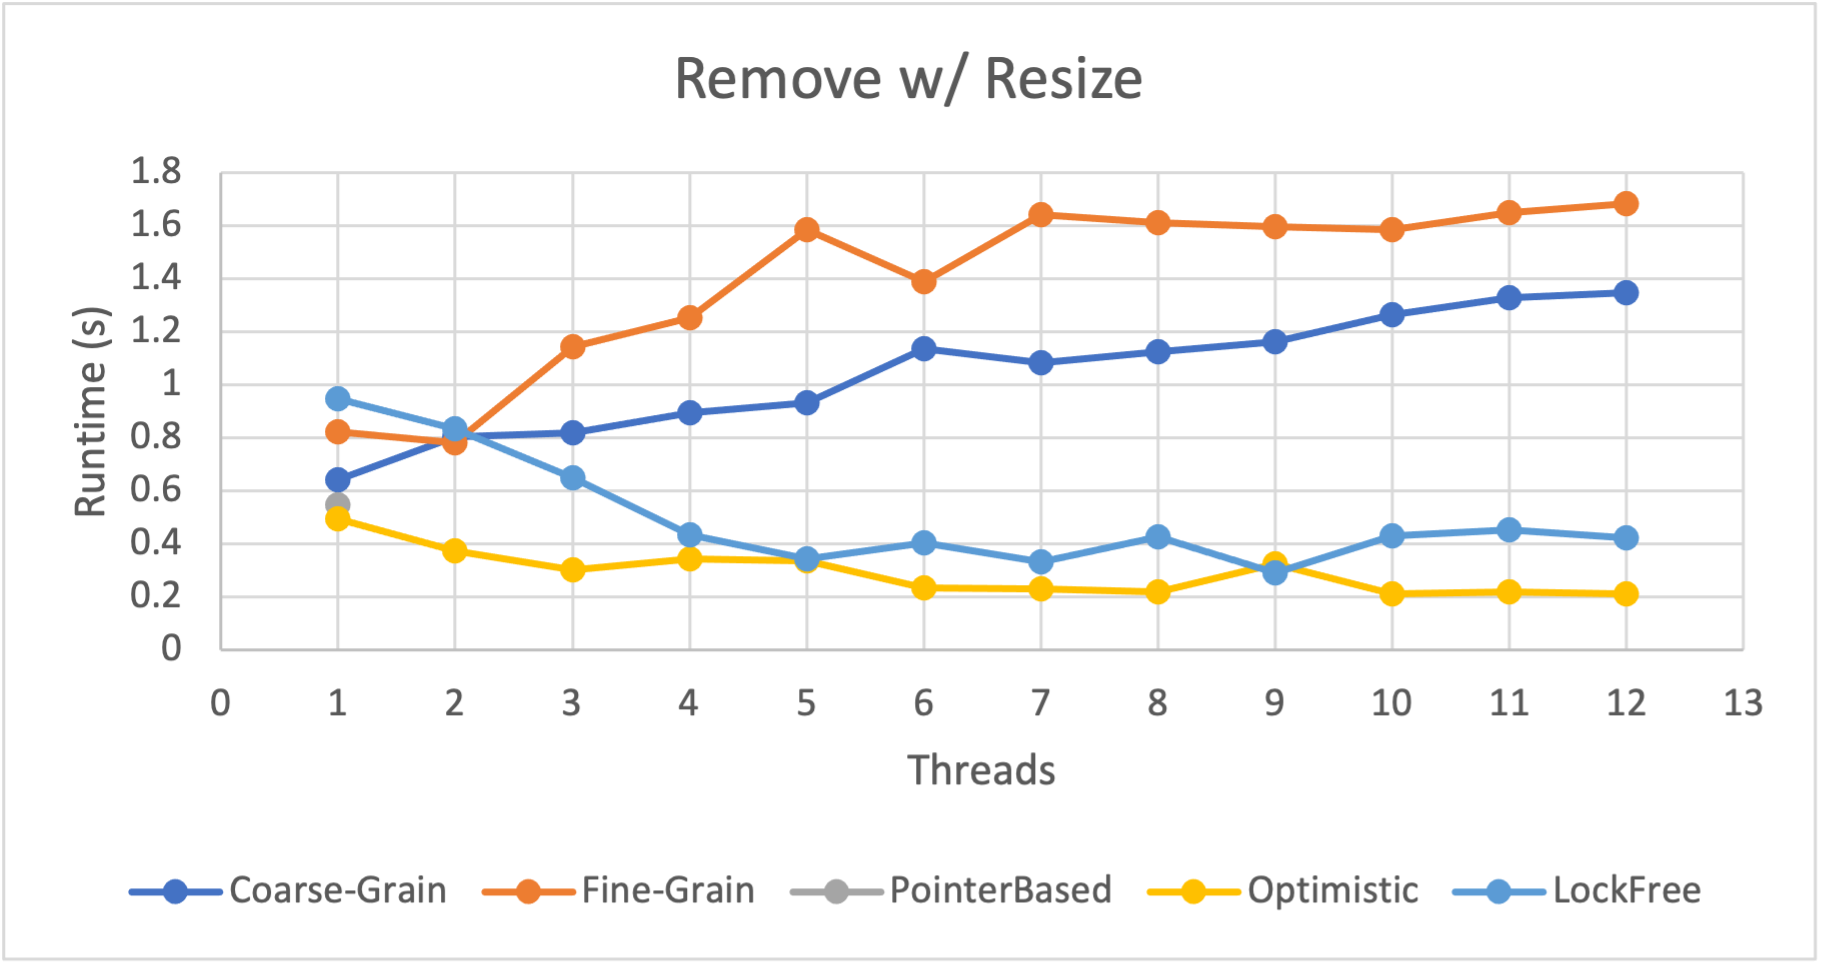
\includegraphics[width=\textwidth]{V1Remove.png}
		\caption{Removals Only}
		\label{fig:fig1a}
	\end{subfigure}
	\begin{subfigure}{.5\textwidth}
		\includegraphics[width=\textwidth]{V1Insert.png}
		\caption{Insertions Only}
		\label{fig:fig1b}
	\end{subfigure}
	\begin{subfigure}{.5\textwidth}
		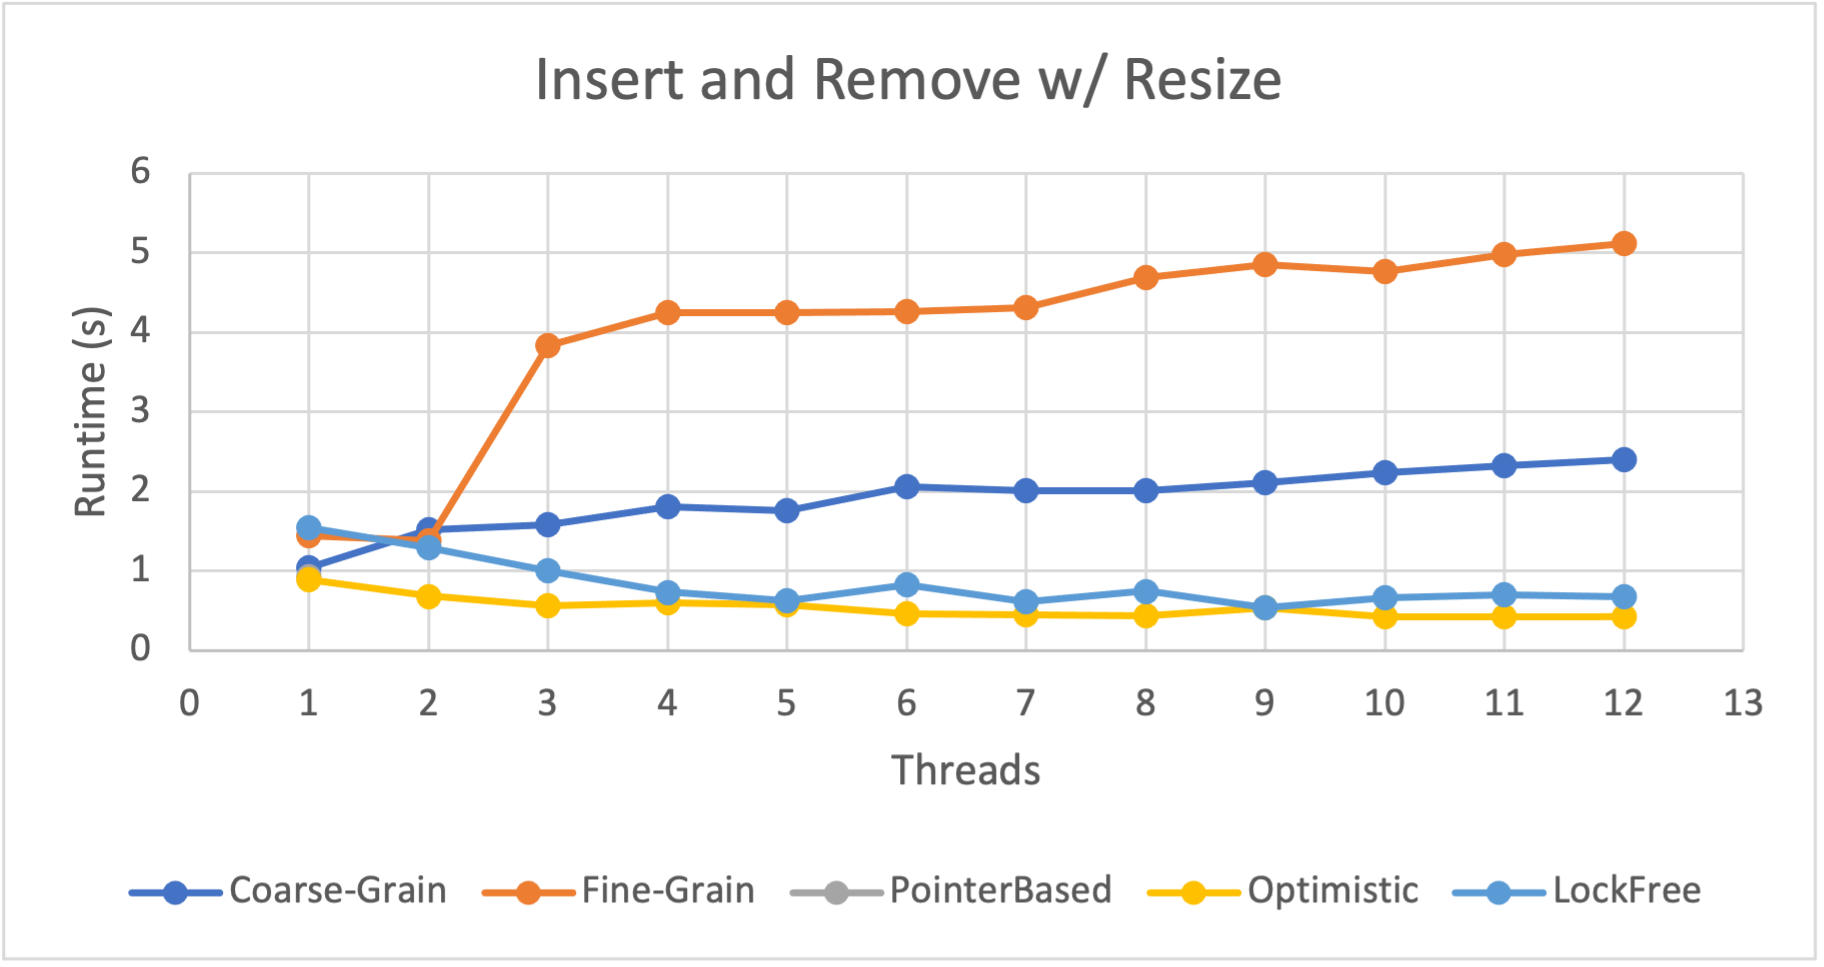
\includegraphics[width=\textwidth]{V1InsertRemove.png}
		\caption{Removal and Insertions Mixed}
		\label{fig:fig1c}
	\end{subfigure}
    \caption{Removal, insertion, and mixed operations test for the resizable octree version.}
    \label{fig:fig1}
    
\end{figure}

\subsection{Resizable Octree} %V1
These first set of results involved testing the concurrency of octrees that needed to be resized.
\subsubsection{Removal}~\\
\indent \indent As depicted in Figure \ref{fig:fig1a}, for most of the tests we ran involving removal, optimistic performed better than lock-free, while the coarse-grained and fine-grained algorithms increased runtime when the number of threads increased as well. Compared to a pointer-based sequential approach, we reported a speed-up of about 2.6 times using the optimistic approach with twelve threads.

\subsubsection{Insertion}~\\
\indent \indent As can be seen in Figure \ref{fig:fig1b}, for insertion, the best performing algorithm varied between lock-free and optimistic depending on the number of threads used. Ultimately, optimistic outperformed lock-free while both saw decreasing runtime with the number of threads increasing. Compared to a pointer-based sequential approach, we reported a speed-up of roughly 4.5 times using the optimistic approach with twelve threads.

\subsubsection{Mixed Operations}~\\
\indent \indent As shown in Figure \ref{fig:fig1c}, both the optimistic and lock-free approaches performed similarly when testing them with mixed operations, but in the end, the optimistic synchronization performed better than lock-free. Once again, we see an increase in runtime for the coarse-grained and fine-grained approaches when the number of threads being used increase. Compared to a pointer-based sequential approach, we reported a speed-up of just over 2.2 times using the optimistic approach with twelve threads.

\begin{figure}[h!]
    \centering
    \begin{subfigure}{.5\textwidth}
		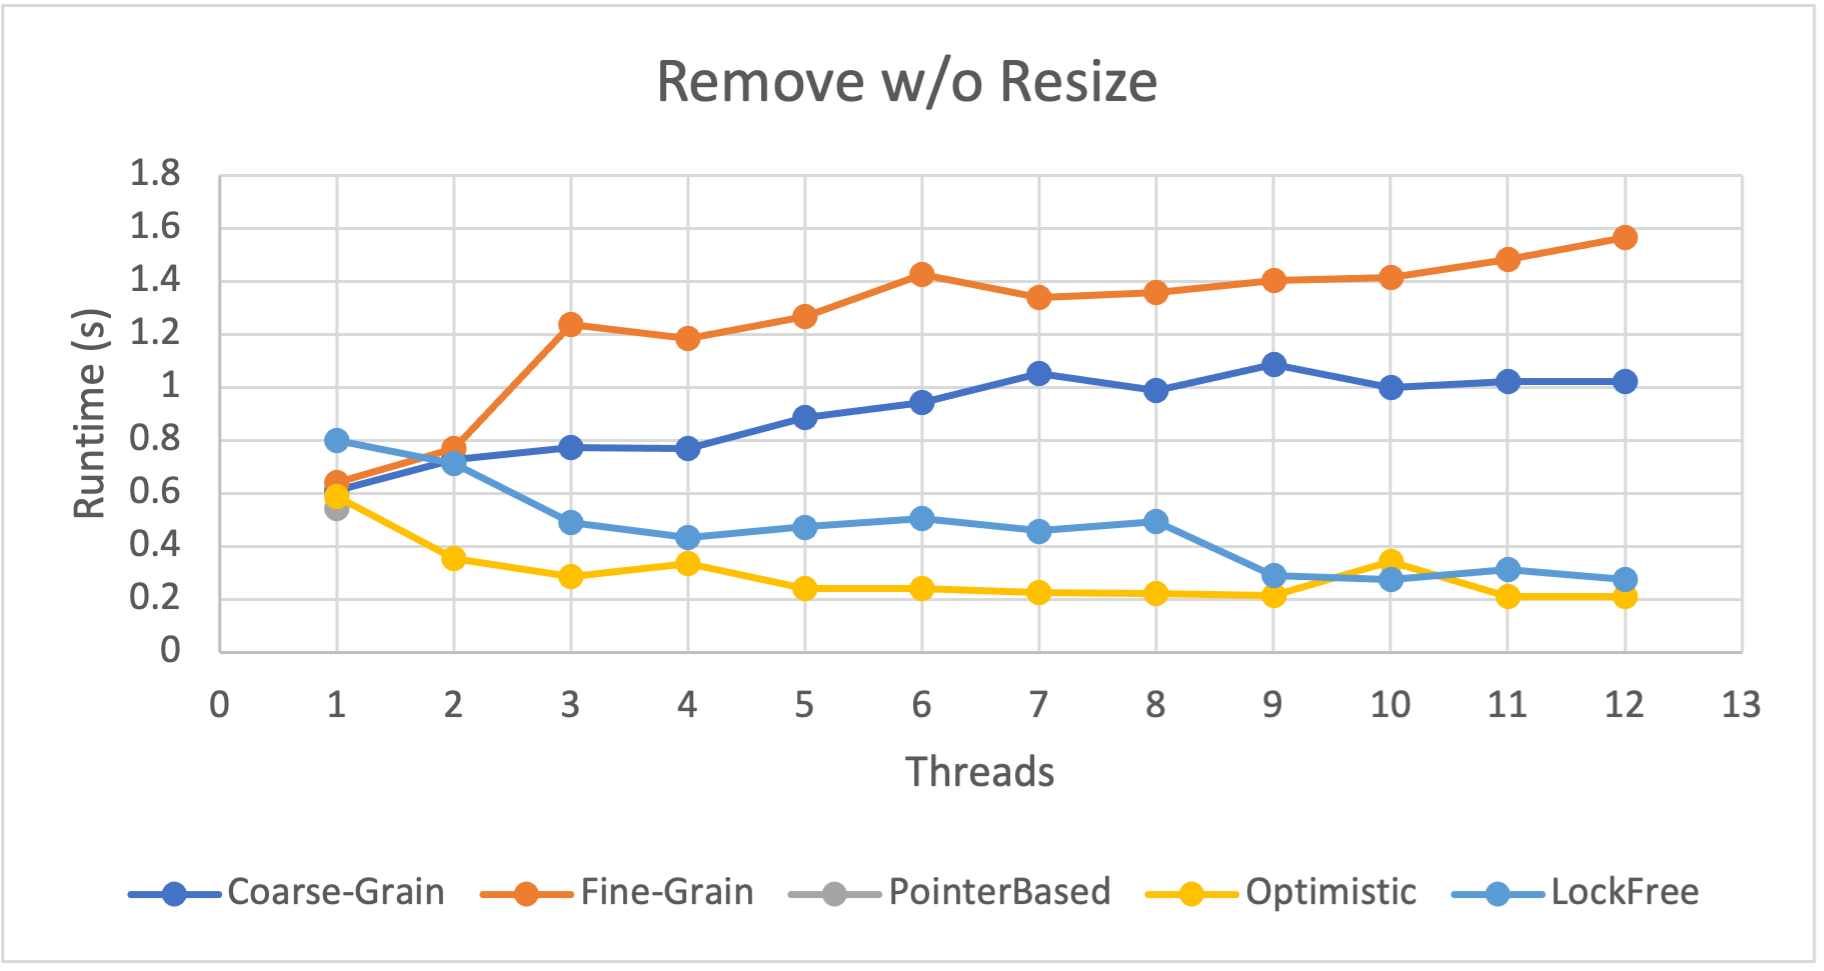
\includegraphics[width=\textwidth]{V2Remove.png}
		\caption{Removals Only}
		\label{fig:fig2a}
	\end{subfigure}
	\begin{subfigure}{.5\textwidth}
		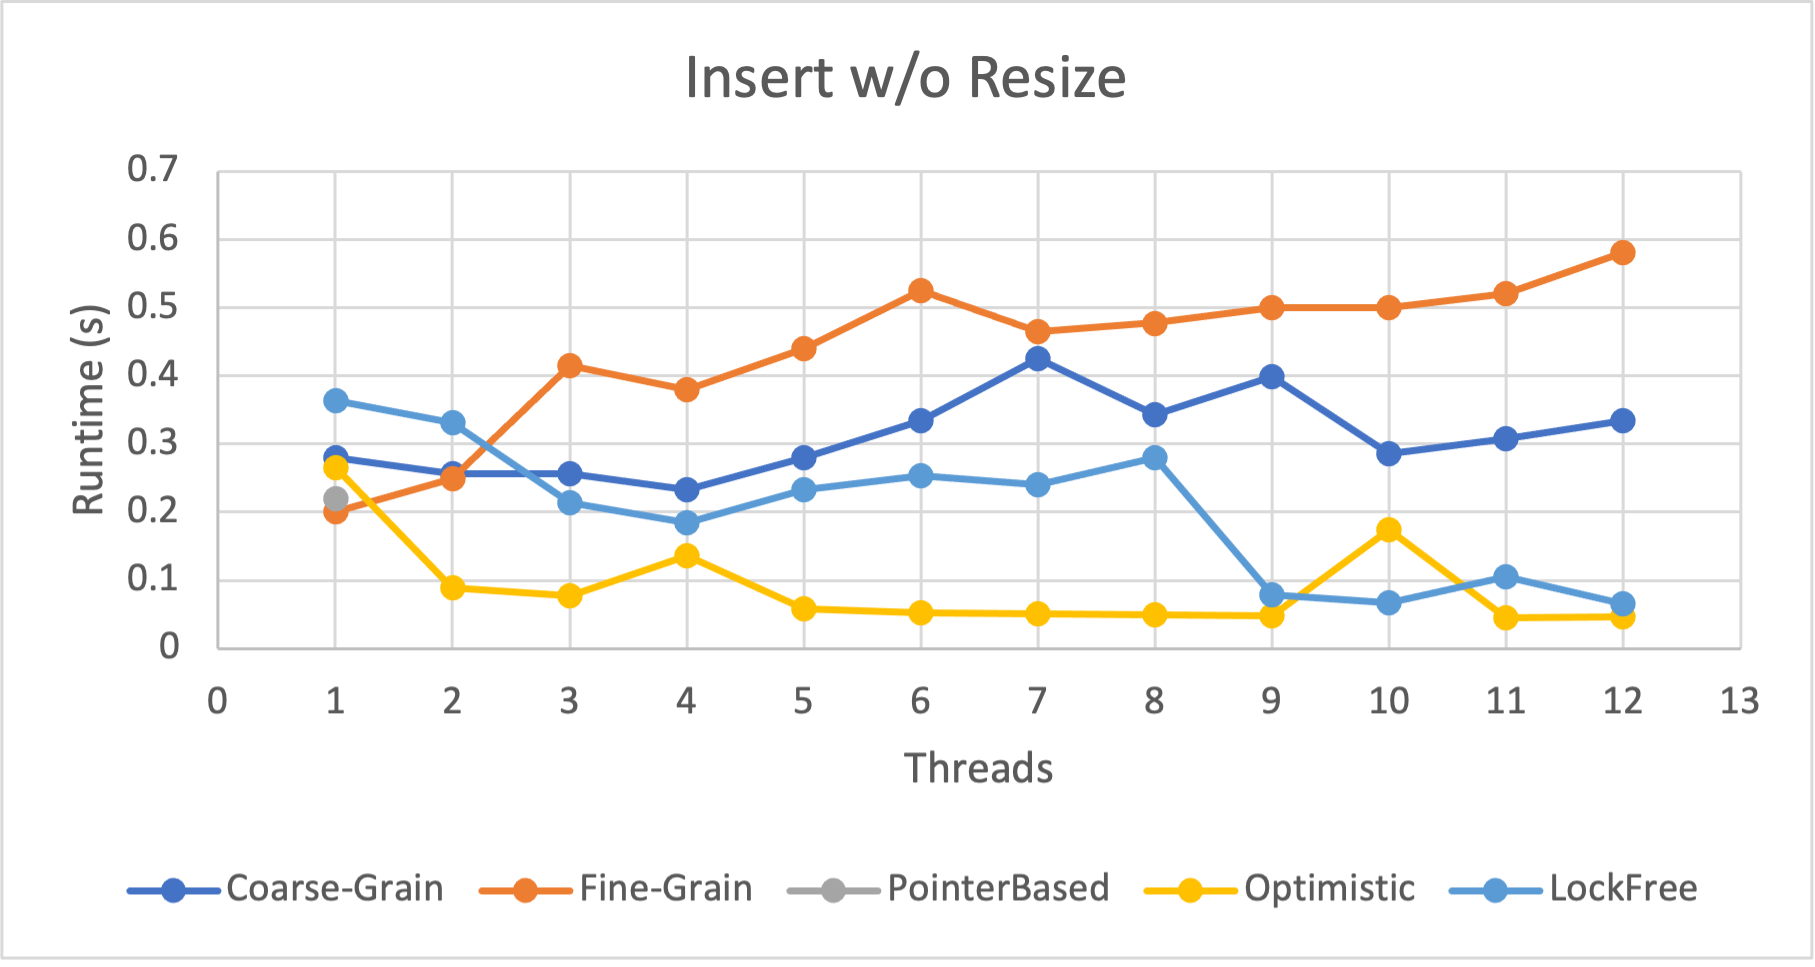
\includegraphics[width=\textwidth]{V2Insert.png}
		\caption{Insertions Only}
		\label{fig:fig2b}
	\end{subfigure}
	\begin{subfigure}{.5\textwidth}
		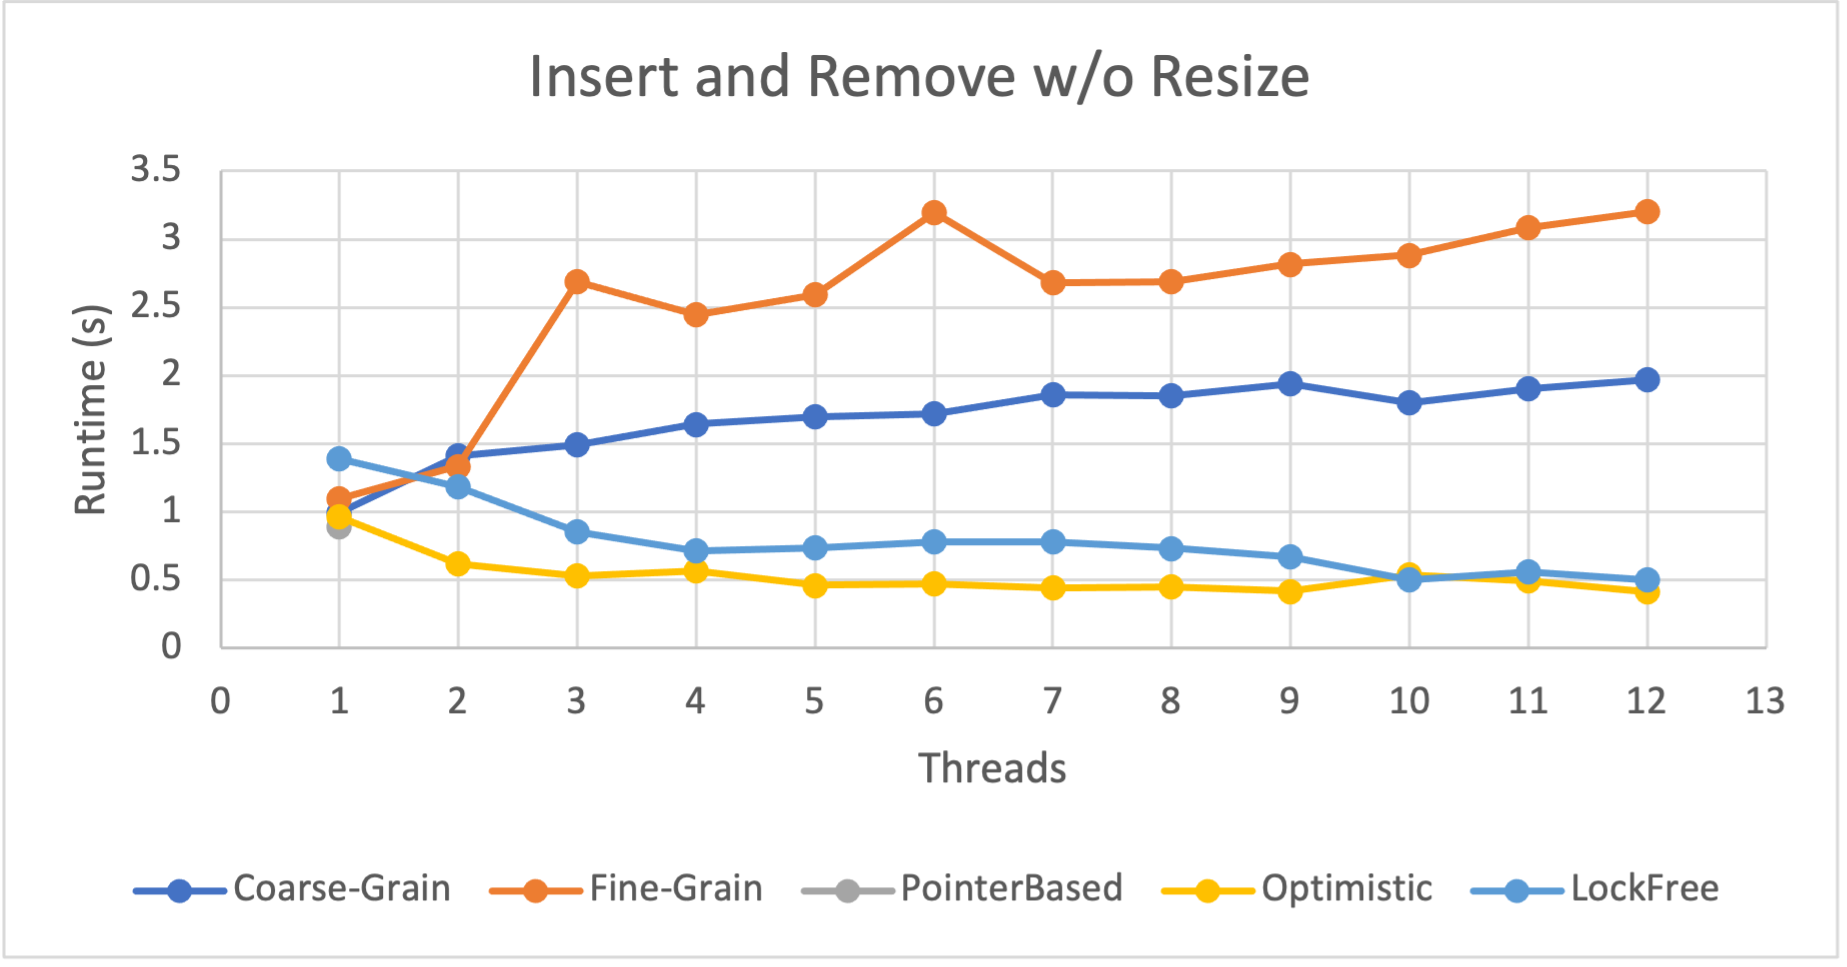
\includegraphics[width=\textwidth]{V2InsertRemove.png}
		\caption{Removal and Insertions Mixed}
		\label{fig:fig2c}
	\end{subfigure}
    \caption{Removal, insertion, and mixed operations test for the non-resizable octree version.}
    \label{fig:fig2}
    
\end{figure}

\subsection{Bounded Octree} %V2
The following results involved testing the concurrency of octrees that had precomputed bounds.
\subsubsection{Removal}~\\
\indent \indent In terms of removal, the optimistic approach consistently provided the greatest speedup, regardless of the number of threads. This can be seen in Figure \ref{fig:fig2a}. Overall, the coarse-grained and fine-grained methods slowed down with an increase in the number of threads, but the optimistic and lock-free techniques did see an overall decrease in runtime. Compared to a pointer-based sequential approach, we reported a speed-up of roughly 2.6 times using the optimistic approach with twelve threads.

\subsubsection{Insertion}~\\
\indent \indent As shown in Figure \ref{fig:fig2b}, for insertion, the lock-free and optimistic approaches varied in best performance when the number of threads increased, but ultimately, optimistic performed better in a test with twelve threads. Similar to the removal method, the coarse-grained and fine-grained approaches slowed down with an increase in the number of threads whereas optimistic and lock-free sped up. Compared to a pointer-based sequential approach, we reported a speed-up of about 4.75 times using the optimistic approach with twelve threads.

\subsubsection{Mixed Operations}~\\
 \indent \indent When it came to mixing both insertion and removal operations in the octree, our optimistic approach outperformed the lock-free method. This is shown in Figure \ref{fig:fig2c}. However, both optimistic and lock-free performed up to seven times better than the coarse-grained and fine-grained synchronization techniques. Compared to a pointer-based sequential approach, we reported a speed-up of nearly 2.2 times using the optimistic approach with twelve threads.


\section{Conclusion} \label{sec:sec6}
We expected the lock-free implementation to provide the best results with twelve threads. Overall, however, we saw that optimistic had the best performance in both versions of our implementations and in all of the tests performed. There was no significant difference in runtime when testing both resizable and bounded octrees. We also saw similar speedups using the optimistic approach with twelve threads among both versions. 

\subsection{Challenges}
In working through the different algorithm implementations, we faced many roadblocks that we did not initially anticipate. First, as we increased the complexity of the synchronization method, moving from coarse-grained to lock-free, the location of the linearization point for functions became much stricter. When we started the lock-free implementation, we realized that, due to the subdivision algorithm, it was necessary to rework the insert, remove, and contains methods. The methods needed to be able to retry if the node they were operating in was being subdivided while they were doing work. The reason why is because our subdivision algorithm may not see the newly inserted point before reinserting and it may also clear the points list before the remove or contains methods are able to operate on it.

\subsection{Future Research}
For the future, we would like to see comparisons of pointer-based octrees with linear-based octrees and how each implementation performs with the different synchronization techniques we tested. We were also planning on implementing a lazy synchronization. However, we realized we would have to change our removal method entirely, so that it would be able to remove nodes in the octree as well. In the future, we'd like to be able to change our removal method to allow for lazy removal and see how the runtime compares with the others.


\bibliography{COP4520GroupProject}{}
\bibliographystyle{IEEEtran}


\end{document}
